\documentclass[11pt,a4paper]{article}
\usepackage[a4paper,inner=27mm,outer=27mm,top=25mm,bottom=25mm]{geometry}
\usepackage[T1]{fontenc}
\usepackage{amsmath,amsthm}
\usepackage{lmodern,amssymb}
\usepackage{microtype,booktabs,tabularx,array,enumitem,caption,titlesec,needspace,placeins}
\usepackage{tikz}
\usetikzlibrary{arrows.meta,positioning,patterns}
\usepackage[authoryear,round]{natbib}
\usepackage{fancyhdr,tocloft}
\usepackage[colorlinks=true,linkcolor=black,citecolor=blue!50!black,urlcolor=blue!50!black,
  pdftitle={Exact Name-Field Noninterference in Language-Model Screening},
  pdfauthor={Adel Mansour},pdfdisplaydoctitle=true]{hyperref}
\usepackage{bookmark}

\definecolor{ink}{HTML}{17191B}
\definecolor{teal}{HTML}{126B65}
\definecolor{rose}{HTML}{973E30}
\definecolor{soft}{HTML}{EAF5F2}
\definecolor{bluegray}{HTML}{EAF0F5}
\definecolor{charcoal}{HTML}{414D55}
\color{ink}
\setlength{\parindent}{1em}
\setlength{\parskip}{3.5pt plus 1pt}
\setlength{\headheight}{15pt}
\setlength{\emergencystretch}{1.3em}
\renewcommand{\arraystretch}{1.19}
\raggedbottom
\fancyhf{}
\fancyhead[L]{\footnotesize\itshape Exact name-field noninterference}
\fancyhead[R]{\footnotesize\itshape Adel Mansour}
\fancyfoot[C]{\small\thepage}
\renewcommand{\headrulewidth}{0.25pt}
\titleformat{\section}{\Large\bfseries}{\thesection}{0.65em}{}
\titleformat{\subsection}{\large\bfseries}{\thesubsection}{0.65em}{}
\titlespacing*{\section}{0pt}{17pt plus 2pt}{5pt}
\titlespacing*{\subsection}{0pt}{12pt plus 2pt}{4pt}
\setcounter{tocdepth}{2}
\renewcommand{\contentsname}{Table of Contents}
\setlength{\cftbeforesecskip}{4pt}
\setlength{\cftbeforesubsecskip}{1.2pt}
\setlength{\cftbeforefigskip}{5pt}
\setlength{\cftbeforetabskip}{5pt}
\cftsetindents{sec}{0pt}{2em}
\cftsetindents{subsec}{1.7em}{3em}
\captionsetup{font=small,labelfont=bf,labelsep=period,skip=7pt}
\setlist{nosep,leftmargin=1.7em}
\newtheorem{proposition}{Proposition}
\newcommand{\T}{\mathcal{T}}
\newcommand{\E}{\operatorname{Emb}}
\newcommand{\code}[1]{\texttt{#1}}

\begin{document}
\hypersetup{pageanchor=false}
\begin{titlepage}
  \pdfbookmark[0]{Title page}{title-page}
  \thispdfpagelabel{Cover}
  \centering
  \vspace*{38mm}
  {\Large\scshape Technical Research Preprint\par}
  \vspace{15mm}
  {\fontsize{25}{31}\selectfont\bfseries
    Exact Name-Field Noninterference\par
    in Language-Model Screening\par}
  \vspace{12mm}
  \rule{0.42\textwidth}{0.45pt}\par
  \vspace{10mm}
  {\Large Adel Mansour\par}
  \vspace{4mm}
  {\large 16 November 2026\par}
  \vfill
  {\small\href{https://github.com/adelmansourjr/racial-bias-ai-calibration/tree/main/nameguard-paper}{Manuscript, source and research archive}\par}
  \vspace*{12mm}
\end{titlepage}

\pagenumbering{roman}
\hypersetup{pageanchor=true}
\pagestyle{plain}
\newcommand{\frontheading}[1]{%
  \phantomsection
  \section*{#1}%
  \addcontentsline{toc}{section}{#1}}

\frontheading{Abstract}

A language model can give consistent scores across applicant names and still draw the wrong conclusion from a résumé. We study these two failures separately. Our method tokenises and embeds the original named input, then excludes the reviewed name rows from the transformer’s scoring path. For admitted inputs with identical retained tokens, the protected activations, scores and deterministic reports are equal. The guarantee also extends to greedy generation with a fresh cache. In 119 real résumé excerpts evaluated under four names, all protected score vectors and report bytes matched. The unrestricted model changed its binary decision in 18 excerpts. In a public benchmark with human-labelled source support, all 20 generation comparisons across four names passed, but the evidence verifier confirmed 55 of 320 claims, including 19 unsupported claims. A native reference given the identical retained token IDs also reproduced the protected computation. These results establish a precise guarantee about the name field and show why evidence quality requires a separate evaluation.

\medskip
\noindent\textbf{Keywords:} résumé screening, noninterference, activation routing, evidence verification.

\clearpage
\pdfbookmark[0]{Table of Contents}{front-contents}
\tableofcontents

\clearpage
\phantomsection
\addcontentsline{toc}{section}{List of Figures}
\listoffigures
\bigskip
\phantomsection
\addcontentsline{toc}{section}{List of Tables}
\listoftables

\clearpage
\frontheading{Abbreviations and notation}
\begingroup
\small
\noindent\begin{tabularx}{\linewidth}{@{}p{.19\linewidth}>{\raggedright\arraybackslash}X@{}}
\toprule
\textbf{Abbreviation} & \textbf{Meaning} \\
\midrule
A/B & Two answer labels, with their mapping to supported and unsupported reversed between prompts.\\
ARC & AI2 Reasoning Challenge.\\
AUROC & Area under the receiver operating characteristic curve.\\
CV & Curriculum vitae.\\
FEVER & Fact Extraction and VERification.\\
ID & Identifier. In this report, a token ID is its integer vocabulary index.\\
IEEE & Institute of Electrical and Electronics Engineers.\\
ISO/IEC & International Organization for Standardization and International Electrotechnical Commission.\\
KV cache & The keys and values retained by attention between decoding steps.\\
LLM & Large language model.\\
LoRA / QLoRA & Low-rank adaptation and its quantised-base variant.\\
MLX & The Apple Silicon machine-learning framework used in the experiments.\\
NIST & United States National Institute of Standards and Technology.\\
SQuAD & Stanford Question Answering Dataset.\\
\bottomrule
\end{tabularx}

\medskip
\noindent\begin{tabularx}{\linewidth}{@{}p{.19\linewidth}>{\raggedright\arraybackslash}X@{}}
\toprule
\textbf{Symbol} & \textbf{Meaning} \\
\midrule
\(x,\ \T(x)\) & Rendered named prompt and its exact token ID sequence.\\
\(P(x),\ e(x)\) & Retained physical positions and the ordered token IDs at those positions.\\
\(H_\ell(x)\) & Retained hidden state after \(\ell\) transformer blocks.\\
\(N,\ m,\ K,\ X\) & Accepted-set size, audit size, unknown number of errors in that set, and sampled error count.\\
\(U\) & Upper confidence bound on the finite accepted-set error count.\\
\bottomrule
\end{tabularx}
\endgroup

\clearpage
\frontheading{Vocabulary}

\begin{description}[leftmargin=1.1em,labelindent=0pt,labelsep=.55em,style=nextline,itemsep=8pt]
\item[Admission] A request is admitted when its reviewed spans and native token IDs satisfy the contract and scoring can proceed.
\item[Activation] An internal numerical state computed while the model processes a prompt.
\item[Name-field noninterference] Equal protected states and outputs when two admitted prompts differ in the designated name field and retain the same evidence.
\item[Witness] A proposed split at reviewed character boundaries whose separate token sequences reproduce the full prompt's native tokens.
\item[Evidence tuple] The exact ordered sequence of token IDs retained after the reviewed identity span is excluded from the scoring path.
\item[Coverage] The fraction of evaluated claims receiving confirmation. Confirmations count whether or not the reference label supports them.
\item[False-support risk] The fraction of confirmed claims marked unsupported by the reference labels.
\item[Same-ID reference] An ordinary model invocation supplied with precisely the retained token IDs used by the protected path.
\end{description}

\clearpage
\pagenumbering{arabic}
\pagestyle{fancy}


\section{Introduction}

A recruiter can ask a straightforward question of a screening tool. If the qualifications stay fixed, should changing the name on the résumé change the result? Correspondence studies use this intervention to measure discrimination in hiring \citep{bertrand2004}. Similar audits have documented sensitivity to names in language-model screening and retrieval \citep{armstrong2024,wilson2024}. A score gap calculated across two name groups, however, can conceal changes for individual applicants. If two résumés receive decisions \( (1,0) \) under one name condition and \( (0,1) \) under another, both shortlist rates are \(50\%\), even though both applicants exchange outcomes.

Reducing an observed group gap and isolating an input channel are different engineering objectives. A narrower question can be answered exactly. Can a particular model interface enforce that changing one reviewed field leaves the computation unchanged? Evaluation then has two parts. The first checks the intervention against the information-flow property. The second asks how often the resulting system can make a justified decision.

We implement that interface for frozen Qwen2.5-1.5B-Instruct \citep{qwen2024}. It preserves the original named prompt through tokenisation and embedding. Each protected block then operates on the same ordered stream of retained evidence wherever two variants satisfy the token contract. We derive the equality of states and outputs, test it on résumé excerpts and generated evidence reports, and compare it with the ordinary model given the same retained token IDs. We also test two evidence verifiers on a public human-labelled benchmark. Both miss the prespecified risk and coverage target. Publishing those outcomes alongside the proof makes clear what a screening tool can certify about its computation and what it still needs to establish about its judgement.

\section{Related work}
\label{sec:related}

This targeted review covers research on hiring audits, representation editing, information flow, and evidence verification. We prioritise primary publications that define a comparable intervention or interpret one of our measurements. Two directly relevant public preprints are identified as such because they bear on the scope and priority of the contribution. This is a narrative review of methods and assumptions. It does not estimate a pooled effect across hiring studies.

\subsection{Résumé correspondence studies and language-model audits}

\citet{bertrand2004} varied names on otherwise comparable résumés and measured employer callbacks. \citet{kline2022} extended the correspondence design to large U.S.\ employers and documented substantial variation across firms. Both designs make the name cue experimentally useful while leaving the meaning of that cue dependent on the context. Names can carry associations with several aspects of identity, and other résumé content can carry identity cues independently. \citet{kang2016}, for example, studied how applicants altered multiple parts of their résumés to obscure racial cues. \citet{behaghel2015} found that anonymous résumés changed interview and hiring outcomes in their field experiment, with adverse effects for minority candidates among participating firms. Removing a field thus changes the evidence available to a real decision process. Its impact on fairness depends on the decision process that receives the remaining evidence.

The same identification strategy has been applied to language-model screening. \citet{armstrong2024} varied names in GPT-based screening prompts and examined ratings and recommendations. \citet{wilson2024} audited résumé retrieval through embedding similarity, examining race, gender and their intersection. These studies help explain why the model, task and endpoint matter. A retrieval rank can move even when a binary decision at one cutoff does not. A mean score can remain stable while applicants exchange ranks. Our paired outcomes therefore include continuous logits, binary choices and deterministic report bytes. We keep the comparison within each underlying résumé. Changing the name string is an intervention on one cue.

\citet{wolfe2021} showed that name frequency and tokenisation matter when contextual language models represent names. \citet{an2023} explicitly studied how demographic attributes and tokenisation length affect first-name bias estimates. That finding is directly relevant to an inference guarantee. Substituting a longer name can change both the token IDs near a field boundary and the positions used for later evidence. An audit can treat those as nuisance variables. An exact intervention has to specify how they are handled. We report token admission separately and require a common retained sequence for any comparison covered by the proof.

\subsection{Individual invariance, group outcomes and institutional context}

Fairness criteria answer different questions. \citet{hardt2016} define outcomes conditional on the true label for equalised odds and equality of opportunity. Those definitions require credible task labels and a group variable. In the causal framework of \citet{kusner2017}, counterfactual fairness asks how a prediction would change in a world with a different value of a protected attribute. Our intervention keeps every retained token fixed and alters a declared name field. This is an exact statement about the model interface and cannot determine which changes to qualifications, institutions or language would accompany any broader counterfactual. Neither of our datasets provides demographic labels or validated hiring outcomes.

\citet{raghavan2020} connect these measurement choices to the claims vendors make about pre-employment assessments. \citet{selbst2019} explain how narrowing a sociotechnical problem to a model can shift scrutiny away from the institutional processes that generate its inputs and act on its outputs. In our setting, the reviewer who marks a span and the human who handles referrals both influence an applicant's experience. Access to correction, the cost of review, and the distribution of rejected inputs are therefore part of a useful deployment evaluation.

\subsection{Learned invariance and representation editing}

Counterfactual text augmentation constructs paired training examples \citep{zmigrod2019}. \citet{garg2019} study training and evaluation for predictions robust to counterfactual text edits. Paired training can encourage equal decisions on many examples. Its effect has to be tested on edits beyond the training distribution. Parameter-efficient techniques such as LoRA \citep{hu2022}, QLoRA \citep{dettmers2023} and orthogonal fine-tuning \citep{qiu2023} change how a model is adapted. Their adaptation constraints do not themselves specify which of two named prompts must have identical outputs. An earlier subtractive-adapter experiment in our project reduced average logit variation while leaving differences in all 48 tested contexts. The present method uses frozen weights and enforces equality by the inputs supplied to the protected computation.

\citet{ravfogel2020} use iterative nullspace projection to suppress protected information available to linear classifiers. \citet{belrose2023} give an exact linear concept-erasure criterion in closed form. \citet{elazar2021} use removal interventions to investigate whether encoded information affects behaviour. These are useful distinctions for judging a fairness intervention. A good probe can find a signal that a model does not use. A failed probe may have insufficient capacity. A scalar distribution uniform over \(\{-1,1\}\) and one uniform over \(\{-2,2\}\) have the same mean, but the magnitude identifies which distribution supplied any observation. A mean-direction diagnostic therefore gives a narrower claim than an intervention which makes the observed states equal on every admitted pair.

\citet{meade2022} evaluated several debiasing methods and found that gains varied with the bias being measured and could accompany reductions in language-model performance. The public preprint by \citet{karvonen2025} is especially close in application. It evaluates models under more realistic hiring prompts and edits affine concept directions at inference, including experiments where affiliations carry a demographic cue. That approach targets a wider set of signals and reports empirical bias reduction. Our mechanism targets a declared token channel and tests exact equality on that channel. The available experiments have different populations, model settings and endpoints.

\subsection{Information flow, positions and exact baselines}

\citet{goguen1982} formalise noninterference by comparing executions that agree on the information an observer may see. \citet{sabelfeld2003} review how that principle is enforced in programs, and \citet{clarkson2010} formalise properties that refer to sets of execution traces. This is the appropriate model for our claim because a single run cannot establish name-field noninterference. We must compare two runs or prove that their protected inputs and subsequent execution coincide.

Transformer attention \citep{vaswani2017} can mix information across tokens. Rotary position embeddings assign position-dependent rotations to queries and keys \citep{su2024}. Limiting which keys remain visible while retaining original positions can still change the relative distance across a name field. Token pruning methods such as those of \citet{kim2022} also operate on a selected sequence, but choose tokens to preserve task behaviour or improve efficiency. In our setting, token selection follows a reviewed evidence policy and logical positions form part of the proof.

The nearest public mechanism is the serving-time span veto in \citet[Section III]{russinovich2026}, which verifies exact outside-span activations under a fixed-position, same-token-length substitution across multiple model families. It establishes a direct antecedent for exact marked-span isolation. We therefore locate the distinct contribution more narrowly. We define and test a name-field contract that admits unequal name lengths when the same ordered evidence IDs can be preserved, pair it with compact logical execution, and evaluate admission, score equality and evidence quality on the same interface. We include a native reference given identical retained IDs, because that reference should implement the same protected computation. Table~\ref{tab:methods} compares the evidence yielded by selected peer-reviewed methods.

\begin{table}[tbp]
\small
\centering
\caption[Comparison with published methods]{Evidence from selected published methods and the corresponding claim tested here.}
\label{tab:methods}
\begin{tabularx}{\linewidth}{@{}>{\raggedright\arraybackslash}p{.23\linewidth}
 >{\raggedright\arraybackslash}X >{\raggedright\arraybackslash}X@{}}
\toprule
Approach & What the evaluation establishes & What our experiment tests separately \\
\midrule
Correspondence and retrieval audits \citep{bertrand2004,wilson2024}
 & Sensitivity to a manipulated cue in a specified population or ranking task.
 & Exact equality of each admitted pair, including logits and aligned states.\\[2pt]
Counterfactual text training \citep{garg2019}
 & Robustness to evaluated token edits after training.
 & Equality by a deterministic inference contract, with no task-specific weight update.\\[2pt]
Linear representation erasure \citep{ravfogel2020,belrose2023}
 & Suppression of a specified class of decoders or linear concept information.
 & Equality of the full aligned state for each admitted pair after the embedding boundary.\\[2pt]
Question-answering verification \citep{wang2020,fabbri2022}
 & Agreement between a claim and an answer extracted from a document.
 & Whether exact agreement with a supplied span predicts human support labels.\\[2pt]
Selective classification \citep{geifman2017,jones2021}
 & Error as a function of the proportion of cases on which a classifier acts.
 & Separate counts for token admission, confirmation and evidence error.\\
\bottomrule
\end{tabularx}
\end{table}


\subsection{Source verification and selective classification}

SQuAD~2.0 introduced adversarially written unanswerable questions paired with plausible answers \citep{rajpurkar2018}. FEVER separates a claim's verification label from the evidence retrieved in support of that label \citep{thorne2018}. Work on attributed generation likewise measures whether a citation supports its associated statement \citep{gao2023}. These designs arise from a common problem. Locating a plausible span can be easier than judging whether the span answers the question. \citet{wang2020} and \citet{fabbri2022} use question answering to check consistency between a document and a proposed summary. Our candidate-blind verifier tests a restricted version of that idea. It must reproduce an exact proposed answer and verify the source offsets. The human-labelled benchmark then tests the semantic step independently.

Selective classification makes the risk--coverage trade-off explicit \citep{geifman2017}. \citet{jones2021} show that abstention can magnify group disparities. \citet{lee2021} study a group-sensitive selective prediction criterion. \citet{angelopoulos2025} address statistical risk calibration for predictive systems on new examples under their stated assumptions. Our statistical question is different. We sample without replacement from a frozen, finite set of confirmations and verify the audit against its entire labelled census. This avoids relying on an independence assumption about errors within one article. We do not treat four repeated names as four independent confirmations.


\section{Method}
\subsection{Input contract and routing}

Let \(x\) be a named prompt with reviewed character runs, each assigned the role \emph{identity} or \emph{evidence}. Render the fixed chat template once to obtain \(x\), and partition that string into its reviewed runs. Let \(\T\) denote the pinned tokenizer with automatic insertion of special tokens disabled. It is applied to the full string and to each run under the same settings. The runtime checks
\begin{equation}
 \T(x)=\T(r_1)\mathbin{\|}\cdots\mathbin{\|}\T(r_k).
 \label{eq:factor}
\end{equation}
Here \(\|\) denotes sequence concatenation. An exact match witnesses that the reviewed roles can be represented by disjoint groups of native tokens. The runtime also requires a nonempty retained sequence and a retained final readout slot. The compiler may try bounded reassignments of adjacent whitespace, leaving the original string and full token sequence intact. It chooses a reference retained tuple from fitting names by maximising the number of distinct fitting names supported by an admissible split. At inference a matching witness must satisfy Eq.~\ref{eq:factor} and reproduce that tuple exactly. A request outside the contract is referred before scoring. The guarantee is conditional on correct role annotation, so names inside unmarked evidence or mistakes in review remain in scope for separate auditing.

Write \(u=\T(x)\) and let \(P(x)\) index the retained tokens in order. The embedding lookup \(\E(u)\) is evaluated on the full sequence. Only the rows at \(P(x)\) are passed to the transformer blocks. The retained stream uses positions \(0,\ldots,|P|-1\) and a causal mask on that stream. Positions measured in the original prompt would change whenever a name used a different number of tokens. The protected scorer can scatter the aligned states into the original layout with identity slots set to zero for inspection. The cache for greedy generation is built from the packed stream and is fresh for each request. Figure~\ref{fig:routing} traces the two inputs to the common scoring path. Figure~\ref{fig:positions} isolates the position change made by packing.

\begin{figure}[htbp]
\centering
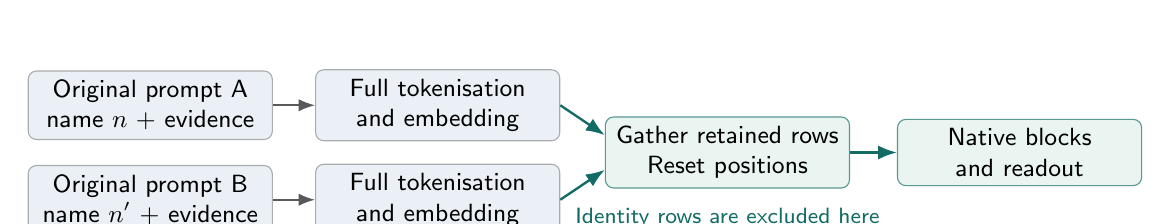
\begin{tikzpicture}[
  font=\small\sffamily, >=Latex,
  box/.style={rounded corners=3pt,draw=ink!36,fill=bluegray,minimum height=8mm,minimum width=31mm,align=center},
  kept/.style={box,draw=teal!70,fill=soft},
  flow/.style={->,draw=ink!72,line width=0.65pt},
  same/.style={->,draw=teal,line width=0.85pt}
]
\node[box] (a) at (0,1.2) {Original prompt A\\name \(n\) + evidence};
\node[box] (b) at (0,0) {Original prompt B\\name \(n'\) + evidence};
\node[box] (ea) at (3.65,1.2) {Full tokenisation\\and embedding};
\node[box] (eb) at (3.65,0) {Full tokenisation\\and embedding};
\node[kept] (gate) at (7.33,0.6) {Gather retained rows\\Reset positions};
\node[kept] (dec) at (11.04,0.6) {Native blocks\\and readout};
\draw[flow] (a.east) -- (ea.west);
\draw[flow] (b.east) -- (eb.west);
\draw[same] (ea.east) -- ([yshift=2.2mm]gate.west);
\draw[same] (eb.east) -- ([yshift=-2.2mm]gate.west);
\draw[same] (gate.east) -- (dec.west);
\node[font=\footnotesize\sffamily,text=teal,align=center] at (7.33,-0.23) {Identity rows are excluded here};

\end{tikzpicture}
\caption[Protected activation path for paired named prompts]{The protected path. The two full prompts may have different token IDs and lengths. When the admitted evidence tuples agree, the transformer sees identical gathered states, positions and masks.}
\label{fig:routing}
\end{figure}

\begin{figure}[htbp]
\centering
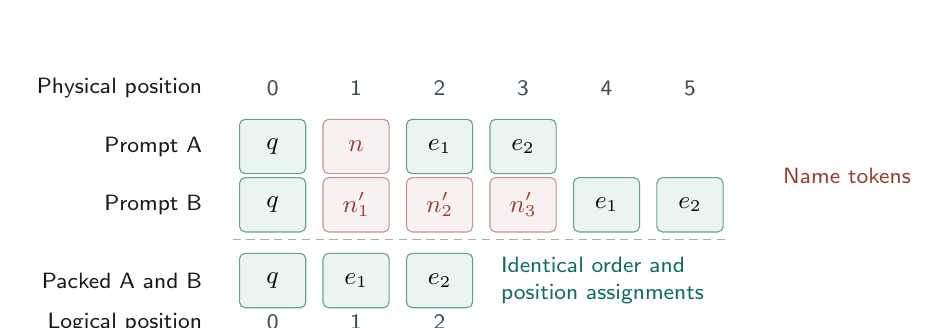
\begin{tikzpicture}[x=1.06cm,y=.74cm,>=Latex,font=\small\sffamily,
    token/.style={minimum width=8.4mm,minimum height=6.9mm,inner sep=1pt,rounded corners=2pt,draw=teal!65,fill=soft},
    identity/.style={token,draw=rose!55,fill=rose!7,text=rose},
    rowlabel/.style={anchor=east,text=ink,align=right,font=\footnotesize\sffamily},
    axis/.style={font=\footnotesize\sffamily,text=charcoal}]
\node[rowlabel] at (-.73,3) {Physical position};
\foreach \i in {0,...,5} {\node[axis] at (\i,3) {\i};}
\node[rowlabel] at (-.73,2) {Prompt A};
\node[rowlabel] at (-.73,1) {Prompt B};
\foreach \p/\t in {0/q,2/e_1,3/e_2} {\node[token] at (\p,2) {\(\t\)};}
\node[identity] at (1,2) {\(n\)};
\foreach \p/\t in {0/q,4/e_1,5/e_2} {\node[token] at (\p,1) {\(\t\)};}
\foreach \p in {1,2,3} {\node[identity] at (\p,1) {\(n'_{\p}\)};}
\draw[densely dashed,ink!35] (-.48,.40) -- (5.48,.40);
\node[rowlabel] at (-.73,-.3) {Packed A and B};
\foreach \p/\t in {0/q,1/e_1,2/e_2} {
 \node[token] at (\p,-.3) {\(\t\)};
 \node[axis] at (\p,-1.02) {\p};
}
\node[rowlabel] at (-.73,-1.02) {Logical position};
\node[anchor=west,align=left,font=\footnotesize\sffamily,text=teal] at (2.62,-.3)
 {Identical order and\\position assignments};
\node[anchor=west,font=\footnotesize\sffamily,text=rose] at (6.00,1.49) {Name tokens};
\end{tikzpicture}
\caption[Physical token positions and packed logical positions]{Why compact positions are part of the guarantee. In this schematic, \(q,e_1,e_2\) are retained tokens. Simply masking the name would leave the distance from \(q\) to \(e_1\) at two positions in prompt A and four in B. Packing makes the distance one in both.}
\label{fig:positions}
\end{figure}


\Needspace{6\baselineskip}
\subsection{Exact noninterference}

For admitted prompts define \(e(x)=u_{P(x)}\). Two prompts are equivalent for scoring when \(e(x)=e(x')\). We compare the retained state in logical token order, rather than comparing physical arrays of potentially different lengths. For a report, fix the additional inputs used by its serialiser, including source text, offsets, rubric and any proposed answer.

\begin{proposition}[Protected-trace equality]
\label{prop:noninterference}
Choose fixed weights, a deterministic execution policy on the packed stream, and fresh per-request decoding state. If two admitted prompts have the same retained ID tuple, their aligned hidden states and readout logits are equal. Deterministic greedy decoding with the same tie and stopping rules gives the same tokens. A deterministic report using identical additional inputs has the same bytes.
\end{proposition}

\begin{proof}
The embedding lookup is row-wise. Gathering the rows whose token IDs form \(e(x)\) therefore gives \(H_0(x)=\E(e(x))\). Write \(L=|e(x)|\), \(\rho_L=(0,\ldots,L-1)\), and \(C_L\) for the causal mask on that sequence. Block \(\ell\) computes
\[
 H_{\ell+1}(x)=F_{\ell,\theta}\bigl(H_\ell(x),\rho_L,C_L\bigr).
\]
The two prompts share \(H_0\), \(L\), \(\rho_L\) and \(C_L\). Induction gives equality through each block, final normalisation and vocabulary projection. The decode prefill uses the same packed inputs and gives equal logits and cache states. Greedy decoding selects the same token, appends it at the same position and updates equal caches in the same way. Induction over decoding steps gives equal continuation tokens until the common stop. The report serialiser then receives identical inputs and emits identical bytes.
\end{proof}

The execution policy must agree for the two packed streams, including precision, kernel and batching behaviour where these affect the numerical result. The implementation is checked on the pinned runtime. A configuration that selects a different scoring kernel from the original physical name length would require a separate proof or conformance test.

A native model given the same retained token IDs is a strong control. Its active input is the same as the protected stream. This equivalence is part of the method's specification and an empirical check of its implementation. Internal routing matters when the original named input must reach the model front end and the protected boundary must be observable. Character-level deletion can produce different token IDs after retokenisation, so it controls a different input transformation. The proof concerns the protected computation. Raw embeddings, identity positions, timing and other outputs outside that path remain outside the observable.

\section{Evaluation design}

Table~\ref{tab:studies} summarises the study units. The tests address input admission, paired equality and evidence quality at different levels.

\begin{table}[htbp]
\small
\centering
\caption[Evaluation units and their endpoints]{Evaluation units and the claims they support. A question or CV condition remains one unit after name substitution.}
\label{tab:studies}
\begin{tabularx}{\linewidth}{@{}>{\raggedright\arraybackslash}p{.23\linewidth}
 >{\raggedright\arraybackslash}p{.29\linewidth} >{\raggedright\arraybackslash}X@{}}
\toprule
Study & Material and unit & Main outcome \\
\midrule
Name admission & 24 held-out names, eight constructed layouts & Compatible token boundaries and shared evidence IDs.\\[2pt]
Synthetic scoring & 32 constructed credential conditions, six names each & Native and protected readout, same-ID reference, credential-task accuracy.\\[2pt]
Résumé text & 119 distinct excerpts, four names each & Exact scoring and reporting. Tool-use labels from one AI annotator.\\[2pt]
Public evidence & 144 development, 312 held-out and 320 reserve questions & Source support from official labels. Four-name comparison on 20 fixed cases per test.\\[2pt]
Capability control & 100 fixed ARC-Challenge questions & Full-vocabulary fidelity when every input token is retained.\\
\bottomrule
\end{tabularx}
\end{table}

\subsection{Résumé excerpts}

We used 119 distinct excerpts from a public résumé dataset \citep{resume}. Sampling required a named tool mention and varied the presence of a nearby activity cue. Records from the 12-document development set were excluded. The three disjoint evaluation cohorts contained 48, 35 and 36 excerpts. Each cohort tested a frozen revision of a rule-based verifier. We changed the verifier after inspecting earlier cohorts; the results therefore describe a sequence of evaluations on fresh extracts rather than a comparison of the revisions on the same inputs.

The question was whether the excerpt explicitly reports the applicant personally using the tool in work or a project. A single AI research annotator who did not see predictions for the upcoming cohort supplied reference judgements before each run. This supports an audit of the experimental rubric. The labels lack independent human adjudication. The candidate name was then changed across four previously unused evaluation strings, yielding 476 requests. We counted model admission, exact protected scores and report bytes, and sampled aligned activation arrays. The ordinary model received the original named prompt as a control. The source verifier identified exact offsets in the excerpt and produced a binary support or review outcome. We also measured a stricter rule requiring both an accepted span and the model's support preference.

\subsection{Public evidence benchmark}

We constructed matched cases from the official SQuAD~2.0 development release. Each selected paragraph supplied one answerable question with its gold answer and one unanswerable question with its human-written plausible answer. Both candidate answers had to occur verbatim at their source offsets. The questions within a pair differ. Matching on paragraph controls the source text and makes string presence uninformative by design (Figure~\ref{fig:benchmark}). The benchmark contains 144 development questions, 312 initial held-out questions and 320 reserve questions. Entire articles were assigned to splits before inference. Protocol and source hashes were recorded locally. No third party registered the plans.

The \emph{candidate-aware} verifier saw the passage, question and proposed answer. We used the signed support margin from each of two complementary label maps. If the margins are \(s_1\) and \(s_2\), their mean cancels a fixed additive A-versus-B logit offset shared by the two maps. This cancellation does not extend to prompt-dependent changes in semantic margins. The minimum requires both margins to clear the cutoff. We fit the lowest cutoff for each of the single, mean and minimum scores that accepted at least 12 development cases with at most \(4\%\) observed false support. The primary rule selected whichever of mean and minimum accepted more cases, with ties going to the mean. When no cutoff qualified, the rule referred every case.

After the development failure, we froze a second protocol and tested it on the unused reserve articles. The \emph{candidate-blind} verifier generated a short answer from the passage and question. It was given neither the candidate answer nor its offset during generation. Let \(g\) be the terminated, single-line model answer after stripping outer whitespace and paired quotation marks, \(a\) the proposed answer, and \(p[i:j]\) the supplied source slice. The verifier confirmed a claim if \(g=a=p[i:j]\) and \(g\) was neither empty nor the abstention sentinel. This test verifies exact agreement with the supplied quote. Whether the quote answers the question remains an empirical issue.

\begin{figure}[htbp]
\centering
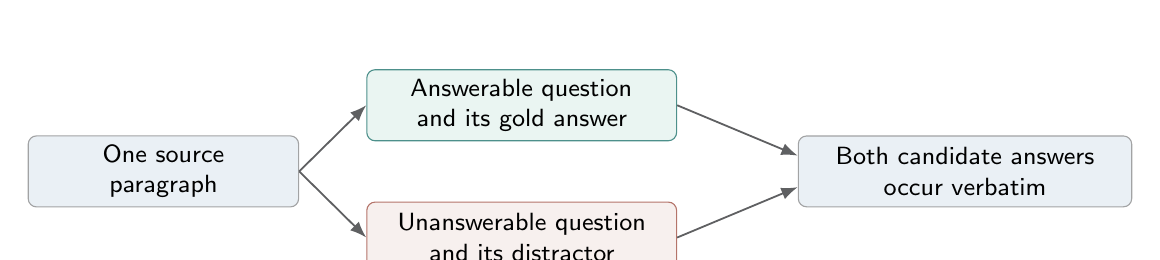
\begin{tikzpicture}[
  font=\small\sffamily, >=Latex,
  box/.style={rounded corners=3pt,draw=ink!40,fill=bluegray,minimum height=9mm,align=center},
  supportedcase/.style={box,draw=teal!75,fill=soft},
  distractorcase/.style={box,draw=rose!72,fill=rose!8},
  line/.style={->,draw=ink!69,line width=0.65pt}
]
\node[box,text width=32mm] (source) at (0,0) {One source\\paragraph};
\node[supportedcase,text width=37mm] (positive) at (4.55,0.84) {Answerable question\\and its gold answer};
\node[distractorcase,text width=37mm] (negative) at (4.55,-0.84) {Unanswerable question\\and its distractor};
\node[box,text width=40mm] (test) at (10.18,0) {Both candidate answers\\occur verbatim};
\draw[line] (source.east) -- (positive.west);
\draw[line] (source.east) -- (negative.west);
\draw[line] (positive.east) -- ([yshift=2mm]test.west);
\draw[line] (negative.east) -- ([yshift=-2mm]test.west);
\end{tikzpicture}
\caption[Construction of the matched evidence benchmark]{The matched-evidence benchmark. Each paragraph supplies a supported and an unsupported candidate for two distinct questions. A literal occurrence check treats them alike.}
\label{fig:benchmark}
\end{figure}


\subsection{Risk, coverage and checks}

Coverage is the number of confirmed cases divided by the number of eligible queries. False-support risk is the fraction of confirmed cases labelled unsupported. If no case is confirmed, risk among confirms is undefined. The prespecified gate required at least \(20\%\) coverage, a one-sided \(95\%\) audit upper bound on false-support risk of at most \(10\%\), and exact conformance on all planned name groups.

The audit estimates the unknown number \(K\) of unsupported claims in the \(N\) accepted items as if only a subset could be reviewed. We fixed a uniform random order of the held-out cases before inference, restricted it to the frozen accepted set, and audited the first \(m=\min(160,\lceil 0.8N\rceil)\) items. Restriction to any fixed accepted subset preserves uniform relative order if the rule is independent of the draw. Conditional on the realised accepted set and its labels, the count \(X\) of audited errors is hypergeometric. For an observed \(x\), we invert the lower tail to compute the upper count
\begin{equation}
 U=\max\left\{K\in[x,N-m+x] :
 \frac{\displaystyle\sum_{i\le x}\binom{K}{i}\binom{N-K}{m-i}}
 {\binom{N}{m}}>0.05\right\}.
 \label{eq:audit}
\end{equation}
Only feasible terms are included. If the true \(K\) exceeds the reported bound, then its lower-tail probability at the observed count is at most \(0.05\). The discrete lower-tail probability at a draw from its own distribution is super-uniform, so this event occurs with probability at most \(0.05\) under repeated audit sampling from the fixed set. We divide \(U\) by \(N\) and compare it with the exhaustive benchmark count. The bound concerns this finite accepted set. It requires no independent-error assumption across claims in the same article and gives no interval for future hiring outcomes.

We ran all inference on a pinned four-bit Qwen2.5-1.5B-Instruct checkpoint using Apple MLX. The checkpoint files and parameter fingerprint were checked. Twenty preselected cases in each public test received four names for conformance. We compare exact values or recorded digests as specified below. Repeated names test counterfactual equality and are counted once per underlying claim in the statistical audit.

\section{Results}
\subsection{Name-field invariance on résumé text}

All 476 named requests were admitted. For all 119 excerpts, protected score vectors and report bytes were identical across names, with 1,488 sampled aligned activation comparisons matching bit for bit. The unrestricted model's score vector changed in every excerpt and its binary decision changed in 18. This comparison measures the causal effect of an experimental change to the name string with evidence fixed. It supplies no demographic classification of the applicant.

The final 36-excerpt cohort illustrates the difference between invariance and task performance. The verifier found four of the seven cases labelled supported and made two unsupported confirmations. Requiring model agreement reduced the final cohort to two correct confirmations and zero unsupported confirmations. It recovered only two of seven supported cases. On the preceding 35-excerpt cohort, the agreement rule still made two unsupported confirmations. Table~\ref{tab:cv-evidence} gives the three cohort outcomes. Every emitted span could be recovered at its exact source offset. The errors concerned whether the applicant performed the activity the quote described.

\begin{table}[htbp]
\small
\centering
\caption[Evidence confirmations across résumé cohorts]{Real résumé evidence verification before applying model agreement. The three rows use successive verifier revisions on disjoint excerpts. The reference labels are from one output-blinded AI annotator.}
\label{tab:cv-evidence}
\begin{tabular}{@{}lrrrr@{}}
\toprule
Cohort & Excerpts & Labelled supported & Correct confirms & Unsupported confirms \\
\midrule
Conservative grammar & 48 & 17 & 7 & 0 \\
Expanded grammar & 35 & 12 & 5 & 2 \\
Attribution guards & 36 & 7 & 4 & 2 \\
\bottomrule
\end{tabular}
\end{table}


\subsection{Human-labelled evidence}

The candidate-aware verifier found no admissible development cutoff and referred all 312 initial test claims, despite area under the receiver operating characteristic curve of \(0.790\), \(0.761\) and \(0.769\) for the single, mean and minimum margins. All 20 name groups matched protected logits and report digests in both maps, and all 3,720 cross-name stage digests matched. A raw binary choice in the unrestricted first map changed with the name in one group. The fully referred rule is operationally uninformative, which is why the protected logits and activation comparisons matter.

The candidate-blind verifier confirmed 55 of 320 reserve claims. Of those, 36 were supported and 19 were unsupported. Coverage was \(17.2\%\) and false-support risk was \(34.5\%\). The audit found 15 unsupported claims in 44 sampled confirmations, giving \(U=22\) and a \(95\%\) upper bound of \(22/55=40.0\%\). The exhaustive count of 19 lay below that bound. The verifier missed both operational thresholds and passed exact name conformance. Figure~\ref{fig:results} compares the operating points on the same cases. At matched coverage, the retrospectively selected top 55 candidate-aware margins gave 11 unsupported confirmations. That comparison shows that withholding the candidate was insufficient. Its cutoff was chosen after inference, so it supplies no validated operating point.

\begin{figure}[!htbp]
\centering
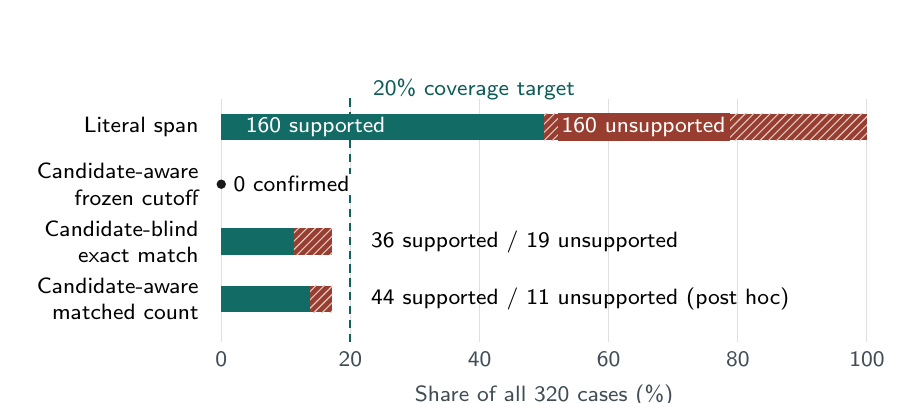
\begin{tikzpicture}[font=\footnotesize\sffamily,x=0.082cm,y=0.70cm]
\foreach \x in {0,20,40,60,80,100} {
  \draw[ink!14] (\x,0) -- (\x,4.4);
  \node[below,text=charcoal] at (\x,0) {\x};
}
\draw[teal!90!black,densely dashed,thick] (20,0) -- (20,4.5);
\node[anchor=west,text=teal!85!black] at (22,4.59) {20\% coverage target};
\node[anchor=east,align=right] at (-2,3.9) {Literal span};
\node[anchor=east,align=right] at (-2,2.86) {Candidate-aware\\frozen cutoff};
\node[anchor=east,align=right] at (-2,1.82) {Candidate-blind\\exact match};
\node[anchor=east,align=right] at (-2,0.78) {Candidate-aware\\matched count};
\foreach \y/\a/\b in {3.9/50/100,1.82/11.25/17.1875,0.78/13.75/17.1875} {
  \fill[teal] (0,\y-.24) rectangle (\a,\y+.24);
  \fill[rose] (\a,\y-.24) rectangle (\b,\y+.24);
  \fill[pattern=north east lines,pattern color=white!70!rose] (\a,\y-.24) rectangle (\b,\y+.24);
}
\fill[ink] (0,2.86) circle[radius=1.7pt];
\node[anchor=west,fill=white,inner sep=1pt] at (1.4,2.86) {0 confirmed};
\node[anchor=west] at (21.7,1.82) {36 supported / 19 unsupported};
\node[anchor=west] at (21.7,0.78) {44 supported / 11 unsupported (post hoc)};
\node[anchor=west,text=white] at (2.3,3.9) {160 supported};
\node[anchor=west,fill=rose,inner sep=1.5pt,text=white] at (52,3.9) {160 unsupported};
\node[below=12pt,text=charcoal] at (50,0) {Share of all 320 cases (\%)};
\end{tikzpicture}
\caption[Coverage and unsupported confirmations on the reserve set]{Reserve-set coverage and its composition. Solid bars represent supported confirmations and hatched bars represent unsupported ones. Both model-based rules failed to achieve the target combination of coverage and risk. The matched-count comparison was calculated retrospectively.}
\label{fig:results}
\end{figure}

\FloatBarrier

\subsection{Generation and diagnostic controls}

In all 20 reserve name groups, the four protected variants yielded identical generated token IDs, packed embedding prefixes and report bytes. All 375 direct cross-name full-vocabulary step comparisons matched. A native cached model given the identical retained token IDs reproduced all 500 compared vocabulary-step digests. With the original named input, native generated sequences varied in seven groups, although exact confirmation did not change in this small panel. Table~\ref{tab:conformance} aligns the paired outcomes across evaluations.

\begin{table}[htbp]
\small
\centering
\caption[Exact name conformance and unrestricted-model changes]{Paired name conformance. Native changes use the endpoint shown and are counts of underlying cases. Activation checks are nested within cases and should not be pooled as independent observations.}
\label{tab:conformance}
\begin{tabularx}{\linewidth}{@{}>{\raggedright\arraybackslash}p{.23\linewidth}
 >{\raggedright\arraybackslash}X >{\raggedright\arraybackslash}p{.23\linewidth}
 >{\raggedright\arraybackslash}p{.20\linewidth}@{}}
\toprule
Cohort & Protected equality & Internal verification & Native changes \\
\midrule
Résumé scoring
 & \(119/119\) cases, logits and report bytes
 & 1,488 direct activation comparisons
 & \(18/119\) binary choices \\[2pt]
Initial public test
 & \(20/20\) cases, logits and report digests
 & 3,720 stage-digest comparisons
 & \(1/20\) first-map binary choices \\[2pt]
Reserve generation
 & \(20/20\) cases, tokens and report bytes
 & 375 direct vocabulary-step comparisons
 & \(7/20\) generated sequences \\
\bottomrule
\end{tabularx}
\end{table}


In a separate retrospective diagnostic we blanked the passage and measured answer agreement before applying the required source-offset check. One answer matched under blank input and 55 matched with the passage present. All 19 wrong full-passage matches disappeared in the blank condition. Thus the omitted passage mattered even for wrong answers, consistent with the author inspection of attribution, rank, numerical and negation errors. Blank input also changes the prompt and can encourage abstention. This control alone cannot identify the specific evidence that caused a model error.

\subsection{Admission and capability controls}

A separate tokenizer stress panel measured an important boundary of the guarantee. With 24 disjoint test names crossed with eight layouts, the compiled contract with exhaustive witness search admitted 170 of 192 inputs, versus 158 for the greedy contract and greedy search. Holding witness search fixed at exhaustive, changing the contract alone increased admission from 160 to 170. Figure~\ref{fig:admission} separates contract selection from witness search.

\begin{figure}[htbp]
\centering
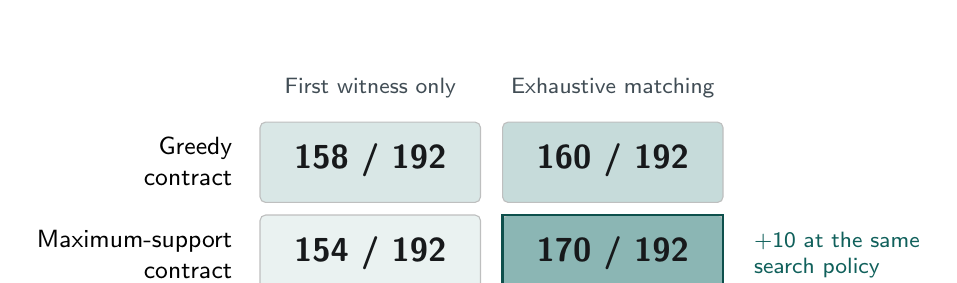
\begin{tikzpicture}[x=1cm,y=1cm,font=\small\sffamily,
 lab/.style={font=\footnotesize\sffamily,text=charcoal,align=center},
 metric/.style={font=\large\bfseries\sffamily,text=ink}]
\node[lab] at (1.4,2.65) {First witness only};
\node[lab] at (4.48,2.65) {Exhaustive matching};
\node[anchor=east,align=right] at (-.23,1.72) {Greedy\\contract};
\node[anchor=east,align=right] at (-.23,.54) {Maximum-support\\contract};
\foreach \x/\y/\n/\tone in {0/1.20/158/16,3.08/1.20/160/24,0/.02/154/9,3.08/.02/170/49}{
 \fill[rounded corners=2pt,teal!\tone!white] (\x,\y) rectangle ({\x+2.8},{\y+1.02});
 \draw[rounded corners=2pt,ink!28] (\x,\y) rectangle ({\x+2.8},{\y+1.02});
 \node[metric] at ({\x+1.4},{\y+.53}) {\n\ / 192};
}
\draw[teal!75!black,thick] (3.08,.02) rectangle (5.88,1.04);
\node[anchor=west,align=left,font=\footnotesize\sffamily,text=teal!90!black] at (6.15,.53)
 {+10 at the same\\search policy};
\end{tikzpicture}
\caption[Admission by contract and witness-search policy]{Factorial admission analysis on 24 held-out names across eight layouts. Each cell gives the number of structurally supported inputs out of 192. The maximum-support contract helps under exhaustive witness search, while pairing it with only the first witness yields the lowest admission count.}
\label{fig:admission}
\end{figure}


On a fixed 100-item ARC-Challenge subset \citep{clark2018}, where every input token was evidence, both the native and protected paths answered 68 items correctly and produced identical full-vocabulary outputs. On a separate synthetic credential diagnostic, native accuracy was 179 of 192 and protected accuracy was 168 of 192. Character deletion also obtained 168. The ARC result establishes all-evidence fidelity. The credential drop limits claims about task usefulness.

\section{Discussion}

An exact citation establishes that a string appears in the source. Screening requires judging whether the source supports the claim and whether the claim is true. The former requires attention to the relationship between the quoted material and the question. The latter may require independent records. Even perfect source reasoning cannot authenticate a credential from the résumé alone. Two applicants can submit the same textual claim while only one has the credential. A text-only procedure necessarily returns the same result in both cases.

The proof covers each new name that satisfies the role and token contract without learning a name-specific correction. Reviewed spans and fixed evidence are essential assumptions. A system that mistakes a name for a skill, misses identifying text elsewhere, or refers more inputs from one naming convention can still disadvantage people. Logging only the protected score would miss those failures.

The work tests one frozen checkpoint and one runtime configuration. The résumé case selection targets particular tools and the semantic labels come from one AI annotator. The public benchmark uses human labels, but its passages concern Wikipedia rather than candidate qualifications. Its balanced case construction fixes the prevalence at one half, and false support among confirmations changes with prevalence. Public examples may also have appeared during pretraining. The study offers no demographic-rate estimate and does not validate an automated hiring process. A deployment evaluation would need independent annotators, job-specific validity evidence, admission rates across naming conventions, and a process for applicants to correct an extraction or appeal a refusal.

\FloatBarrier

\section{Assurance and governance}
\label{sec:assurance}

The model guarantee is useful as one item in a wider evaluation record. \citet{mitchell2019} and \citet{gebru2021} propose model and dataset documentation that specifies intended use, data origin and evaluation boundaries. \citet{raji2020} place those artifacts in an end-to-end auditing process with defined roles and hand-offs. For a screening system, a reviewer needs to see which spans were marked, which configuration ran and why a case was referred. These records also make changes to the model, tokenizer, prompt, contract or hardware identifiable. Resume text and private activation logs need separate access controls because the proof covers the protected computation, not storage.

The NIST AI Risk Management Framework organises risk work around Govern, Map, Measure and Manage \citep{nist100}. Its generative AI profile discusses risks such as confabulation and harmful bias \citep{nist600}. NIST SP~1270 situates bias in systemic, computational and human processes \citep{nist1270}. ISO/IEC~42001 specifies an AI management system, while ISO/IEC~23894 provides guidance on AI risk management \citep{iso42001,iso23894}. IEEE~7003 describes algorithmic bias considerations such as test-data selection and application boundaries \citep{ieee7003}. Table~\ref{tab:assurance} relates the archived tests to these themes. The mapping describes the kinds of evidence a deployment team would need to assemble. The technical prototype has no recorded conformity assessment.

\begin{table}[htbp]
\small
\centering
\caption[Research artifacts and remaining assurance evidence]{Mapping experiment artifacts to assurance questions. These are research artifacts and open deployment questions.}
\label{tab:assurance}
\begin{tabularx}{\linewidth}{@{}>{\raggedright\arraybackslash}p{.20\linewidth}
 >{\raggedright\arraybackslash}p{.35\linewidth} >{\raggedright\arraybackslash}X@{}}
\toprule
Assurance question & Evidence in this study & Evidence a deployment would still need \\
\midrule
Govern and document & Pinned checkpoint, tokenizer policy, experiment hashes, public methods. & Named owners, version approval, incident handling, controlled retention.\\[2pt]
Map the use case & Marked name field, fixed evidence, source-specific rubric. & Job analysis, justified selection criteria, coverage of demographic proxies, accessibility.\\[2pt]
Measure & Paired checks, admission counts, finite error audit, capability controls. & Independently labelled applicant data, outcomes and group-disaggregated admission and errors.\\[2pt]
Manage & Fail-closed referrals and a record of unsupported confirmations. & Review capacity, applicant notice and correction, escalation, re-testing after changes.\\
\bottomrule
\end{tabularx}
\end{table}

For jurisdictional context, New York City's official guidance describes bias audits and notice for covered automated employment decision tools \citep{nyc144}. Annex~III of the EU AI Act lists systems intended for recruitment or candidate selection among its employment use cases \citep{euai2024}. Obligations depend on the intended application and jurisdiction. The results here establish a property of a score path and an evaluated operating point. They supply neither an independent bias audit on applicants nor evidence of legal compliance.


\FloatBarrier

\section{Conclusion}

A precisely marked name field can be prevented from affecting a frozen model's protected states and outputs. The proof holds for identical retained evidence on an admitted request, and the measured equality extends from scores to greedy generation. The evidence-verification results put a concrete limit on what that achievement buys. Removing the name channel still leaves the screening system responsible for reading the source correctly.

\phantomsection
\section*{Code, data and drafting disclosure}
\addcontentsline{toc}{section}{Code, data and drafting disclosure}

The \href{https://github.com/adelmansourjr/racial-bias-ai-calibration/tree/main/nameguard-paper}{manuscript package on GitHub} contains the PDF and editable LaTeX source. The protocols, code, public benchmark identifiers, audit manifests and result summaries are archived in the \href{https://github.com/adelmansourjr/racial-bias-ai-calibration/tree/d51b96f96982bc41a42b368af6d38d459b2a95d5}{project repository at commit \code{d51b96f}}. The \href{https://github.com/adelmansourjr/racial-bias-ai-calibration/tree/main/nameguard-risk-study}{public benchmark package} reproduces the cohort construction and audit. The \href{https://github.com/adelmansourjr/racial-bias-ai-calibration/tree/main/nameguard-real-evidence}{résumé study package} publishes aggregate counts and holds raw excerpts and case-level outputs locally. The \href{https://github.com/adelmansourjr/racial-bias-ai-calibration/tree/main/nameguard-peer-review}{runtime study} documents checkpoint reconstruction and the admission, capability and same-ID controls. OpenAI Codex assisted with drafting, literature search and figure preparation. Study data and result claims refer to the archived experiments.

\clearpage
\appendix
\section{Replication details}
\label{sec:replication}

\subsection{Compiling a common token contract}

For each fitting name \(i\), let \(W_i\) be the set of exact retained ID tuples reachable with a structurally admissible boundary witness. The implementation enumerates permitted adjacent whitespace assignments up to 16 characters per side. It checks token factorisation for each proposed boundary and deduplicates evidence tuples. For every candidate tuple \(e\in\bigcup_i W_i\), it computes
\[
  s(e) = \sum_i \mathbf{1}\{e\in W_i\}.
\]
Any tuple outside the union admits no fitting member, so a maximiser attains the largest structural support possible for one contract on this finite fitting panel. Ties favour lower aggregate formatting cost and then lexicographic order of IDs. A common tuple exists for all fitting names exactly when \(\bigcap_i W_i\) is nonempty. The test name panels are separate from the fit. These are statements about structural feasibility. A runtime witness must also match the approved source roles, and admission on future names remains an empirical question.

\subsection{Run order, public inputs and trace checks}

In the public evidence study, a stable hash orders the 35 eligible articles into eight development, 17 initial test and ten reserve articles. The pipeline keeps paragraphs up to 1,600 characters and excludes embedded chat delimiters. Case construction uses official answerability labels to select matched cases. Those labels are withheld from model inputs and threshold selection on test. Two fixture names compile the contracts, and four evaluation strings are used for the predefined name checks. The first verifier keeps ties together when choosing its cutoff on development. The reserve verifier stops after the specified termination or a 32-token cap. An unterminated or multi-line result is referred.

The pinned generation record uses macOS on arm64, Python 3.12.8, MLX 0.32.3 and MLX LM 0.31.3 \citep{mlxproj}. The \href{https://github.com/adelmansourjr/racial-bias-ai-calibration/blob/d51b96f96982bc41a42b368af6d38d459b2a95d5/nameguard-risk-study/audit/checkpoint-manifest.json}{checkpoint manifest} records full file hashes and the parameter fingerprint. The public replay rebuilds the question IDs, scores the archived predictions against the official labels, checks the planned audit draw and reproduces summary metrics. A separate Metal run can reproduce the inference path with the reconstructed checkpoint. The résumé replay remains limited to released aggregates because raw case material stays local.

\subsection{Fidelity to a name-sensitive baseline}

An invariant replacement cannot preserve every native score if the native scores vary with the name. Given native scalar scores \(v_i\) for one fixed CV, any replacement score \(c\) obeys
\[
  \frac{1}{m}\sum_{i=1}^{m}(v_i-c)^2
   = \frac{1}{m}\sum_{i=1}^{m}(v_i-\bar v)^2+(\bar v-c)^2,
  \qquad
  \min_c\max_i |v_i-c|=\frac{\max_i v_i-\min_i v_i}{2}.
\]
The first identity follows by expanding around the mean. The second follows by placing \(c\) at the midpoint of the two extremal values. These bounds concern agreement with a baseline that may itself depend on the name. Accuracy against an independent label is a separate question, measured in the synthetic credential and source-support experiments.


\clearpage
\renewcommand{\bibfont}{\small}
\setlength{\bibsep}{3.8pt}
\providecommand{\doi}[1]{\href{https://doi.org/#1}{\nolinkurl{#1}}}
\bibliographystyle{plainnat}
\phantomsection
\addcontentsline{toc}{section}{References}
\bibliography{references}
\end{document}
